\chapter{Dynamic Query Expansion}
\markright{Aravindan Mahendiran \hfill Chapter 2. Dynamic Query Expansion\hfill}
\section{Query Expansion}
In most document corpora, a single concept can be referred using multiple terms.
In information retrieval (IR) this is called \emph{synonymy} and has a huge impact on the recall of documents pertaining to the concept.
Researchers address this problem by creating as exhaustive a query as possible. 
But when exploring the Twitter corpora it becomes almost impossible to handcraft such an expansive query as the meme and 
hashtag adaptations are not known {\it a priori}.

To address this issue IR experts use \emph{query expansion} as a key strategy.
Query expansion is a classical technique in information retrieval (IR) ~\cite{manning2008introduction} intended to improve
retrieval performance by overcoming problems such as {\it synonymy}. Query expansion algorithms
are typically iterative in nature wherein a seed set of query terms help identify an initial set
of documents matching the query.
After basic processing (e.g.,
tokenization, stop-word removal and stemming), a richer vocabulary is obtained by ranking the 
terms in these documents by their frequency counts.
The top words from this list are then used to query for documents again. 
This process is continued until no new terms are added to the vocabulary. 

Most query expansion strategies are deterministic.
In contrast to such classical approaches,
our proposed approach is based on a dynamic query expansion strategy  intended to track a vocabulary
over time. Furthermore, unlike most approaches to query expansion, our PSL approach uses a probabilistic formalism
to grow the vocabulary. Finally, PSL provides a rich programmatic environment to incorporate 
multiple indicators (social network, demographics, time) to grow the vocabulary rather than pre-committing to a 
specific strategy.
We first review the PSL framework before proceeding to detail our methodology.

\section{Probabilistic Soft Logic}
Probabilistic Soft Logic ~\cite{kimmig2012short} is a framework for collective probabilistic reasoning on relational domains.
PSL models have been developed in various domains, including collective classification ~\cite{broecheler2010computing}, ontology alignment ~\cite{brocheler2012probabilistic}, personalized medicine ~\cite{bach2010decision}, opinion diffusion ~\cite{bach2012scaling} , trust in social networks ~\cite{huang2012probabilistic}, and graph summarization ~\cite{memory2012graph}.
PSL represents the domain of interest as logical atoms.
It uses first order logic rules to capture the dependency structure of the domain, based on which it builds a joint probabilistic model over all atoms.
Instead of hard truth values of $0$ (false) and $1$ (true), PSL uses soft truth values relaxing the truth values to the interval $[0,1]$.
The logical connectives are adapted accordingly.
This makes it easy to incorporate similarity or distance functions.

User defined \emph{predicates} are used to encode the relationships and attributes and \emph{rules} capture the  dependencies and constraints.
Each rule's antecedent is a conjunction of atoms and its consequent is a disjunction. 
The rules can also labeled with non-negative weights which are used during the inference process. 
The set of predicates and weighted rules thus make up a PSL program where known truth values of ground atoms are set from observed data and unknown truth values for the remaining atoms are learned using the PSL inference mechanism.

Given a set of atoms 
$\ell = \{\ell_1,\ldots,\ell_n\}$,
an interpretation defined as 
$I : \ell \rightarrow [0,1]^n$
is a mapping from atoms to soft truth values.
PSL defines a probability distribution over all such interpretations such that those that satisfy more ground rules are more probable.
\emph{Lukasiewicz t-norm} and its corresponding co-norm are used for defining relaxations of the logical AND and OR respectively to determine the degree to which a ground rule is satisfied.
Given an interpretation $\mathit{I}$, PSL defines the formulas for the relaxation of the logical conjunction ($\wedge$), dis-junction ($\vee$), and negation ($\neg$) as follows:
\begin{align*}
\ell_1 \softand \ell_2 &= \max\{0, I(\ell_1) + I(\ell_2) - 1\},\\
\ell_1 \softor \ell_2 &= \min\{I(\ell_1) + I(\ell_2), 1\},\\
\softneg l_1 &= 1 - I(\ell_1),
\end{align*}  
where we use \textasciitilde to indicate the relaxation of the Boolean domain.
The interpretation $\mathit{I}$ determines whether the rule is satisfied, if not, the \emph{distance to satisfaction}.
A rule $\mathit{r} \equiv \mathit{r_{body}} \rightarrow \mathit{r_{head}} $  is satisfied if and only if the truth value of head is atleast that of the body. The rule's distance to satisfaction measures the degree to which this condition is violated.
\begin{center} 
 $\mathit{d_r}(\mathit{I}) =$ max\{0,$\mathit{I(r_{body}} - \mathit{I(r_{head})}$\}
 \end{center}
PSL then induces a probability distribution over possible interpretations $\mathit{I}$ over the given set of ground atoms $\mathit{l} $ in the domain. 
If $\mathit{R}$ is the set of all ground rules that are instances of a rule from the system and uses only the atoms in  $\mathit{I}$ then,
the probability density function $\mathit{f}$ over $\mathit{I}$ is defined as
\begin{equation}
\label{eq:contimn1}
    f (I) = \frac{1}{Z} \text{exp}[-\sum_{r\in R} \lambda_r (d_r(I))^p]
\end{equation}
\begin{equation}
\label{eq:contimn2}
	Z = \int_{I} \text{exp} [ -\sum_{r\in R} \lambda_r (d_r(I))^p ]
\end{equation}
where~$\lambda_r$ is the weight of the rule~$r$, $Z$ is the continuous version of the normalization constant used in discrete Markov random fields, and ~$p \in \{1, 2\}$ provides a choice between two different loss functions, linear and quadratic.
The values of the atoms can be further restricted by providing linear equality and inequality constraints allowing one to encode functional constraints from the domain.

PSL provides for two kinds of inferences (a) most probable explanation (MPE) 
and (b) calculation of the marginal distributions. 
Given a partial interpretation with grounded atoms based on observed evidence, \emph{most probable explanation} (MPE) inference seeks the truth values for the unobserved atoms satisfying the most likely interpretation. 
%Because energy function is convex, MPE inference is solved using a convex optimization. Because of the structure of the energy function constructed from rules, a fast decomposition algorithm is particularly effective for solving this inference optimization
The MPE inference is a convex optimization problem because the energy function is convex. 
This inference optimization can be efficiently solved using a fast decomposition algorithm ~\cite{bach2012scaling,bach2013hinge} by exploiting the structure of the energy function constructed from rules.
%In MPE inference, given a partial interpretation with grounded atoms based on observed evidence, the PSL program infers the truth values for the unobserved atoms satisfying the most likely interpretation. 
In the second setting, given ground truth data for all atoms we can learn the weights for the rules in our PSL program.
In our work we leverage the MPE inference.

\section{Dynamic Query Expansion using PSL}
In ~\cite{huang2012social}, as part of the same larger project,
PSL was used
to model user affiliations within groups. 
Specifically the authors built a PSL program
for a  social network where they use a set of users, their posts, messages to other users and the various groups they intend to model. 
The rules defined helped capture the dynamics of group affiliations through the various interactions.
Through the MPE inference users were classified into different groups based on their hashtag usage and their interactions with other users.

In this thesis, we extend this earlier work to achieve what we refer to as dynamic query expansion through PSL. 
Similar to the query expansion methodology described earlier, we begin with an initial set of 
hashtags which we believe are indicative of the affinity of a particular user to a candidate 
contesting in the election.
We refer to these hashtags as seed words.
Instead of a single inference, we iteratively perform the inference over successive time windows such that the inference from window $w_t$ is used as a prior to window $w_{t+1}$ and the inference from that is used for window $w_{t+2}$, and so on.
\begin{figure*}[Ht]
	\centering
	%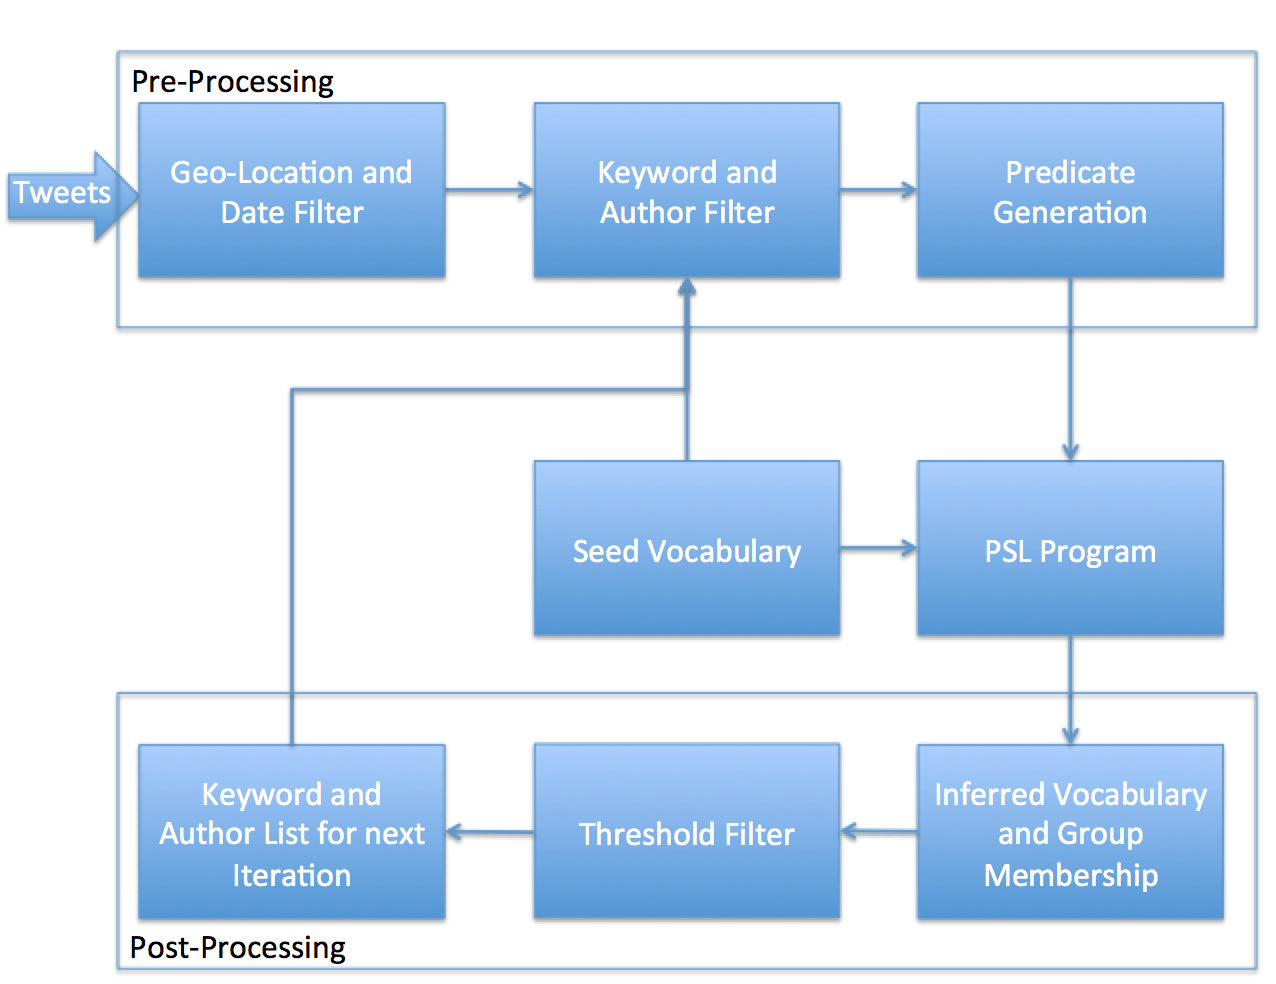
\includegraphics[scale=0.50]{support_files/flowChart.png}
	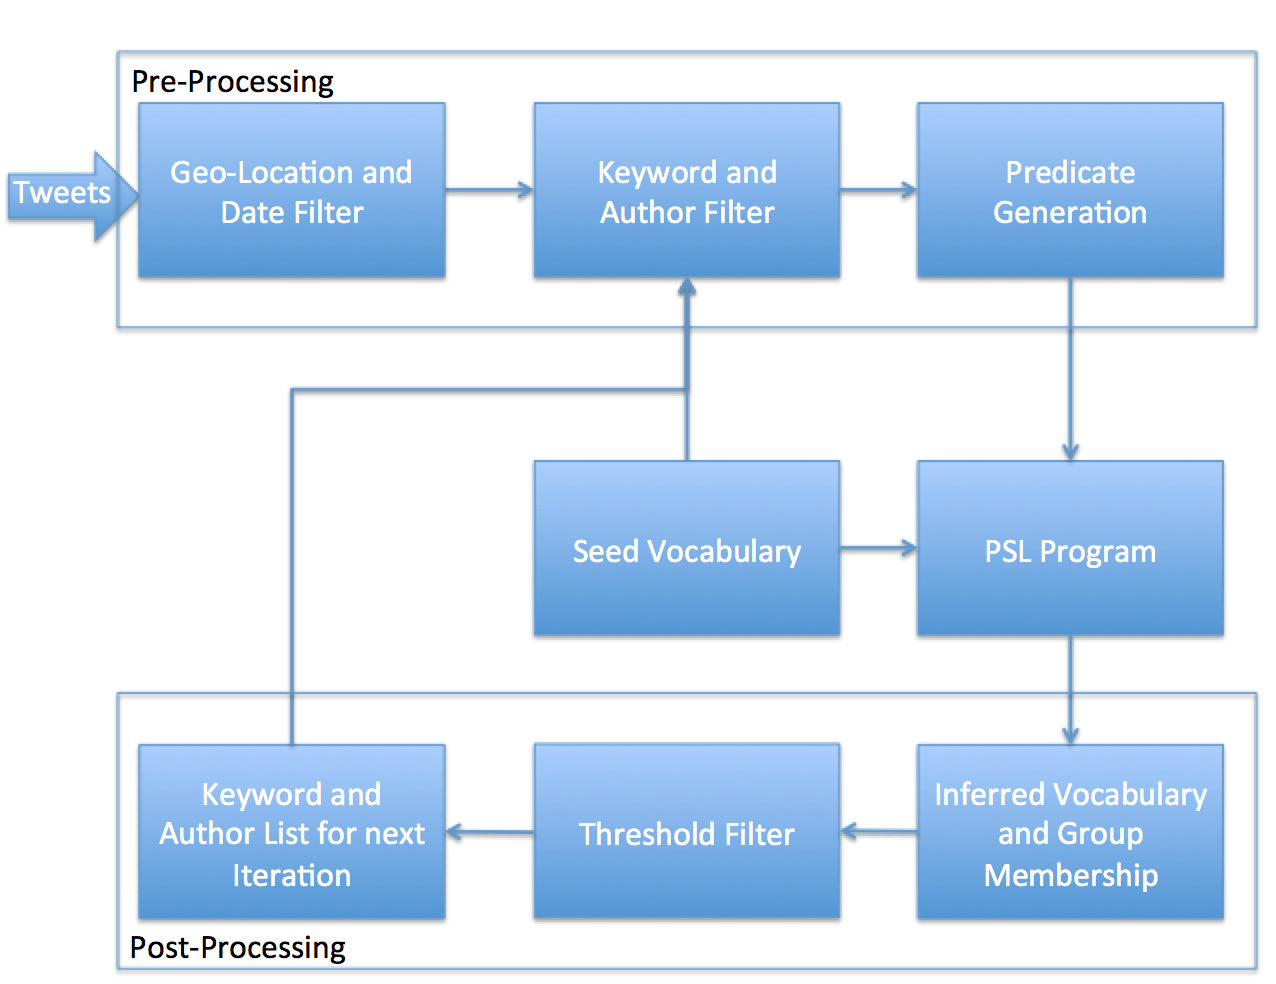
\includegraphics[height=0.5\textheight, width=1.0\textwidth]{support_files/flowChart.png}
	\caption{Design of the query expansion pipeline.}
	\label{fig:flowchart}
\end{figure*}
Figure~\ref{fig:flowchart} illustrates the design of the iterative algorithm for dynamic query expansion.
The initial pre-processing starts with the tweet input stream which is filtered by the date range specified by the window size. 
For each election, tweets from a month leading up to the election were used.
After extensive analysis it was determined that the most optimal window size was three days. 
Smaller window sizes resulted in sub-optimal inferences as there were not enough data points feeding into the PSL stage.
Larger window sizes lead to memory issues as the PSL optimization procedure generates rules by substituting groundings of all possible combinations for the variables in the rules defined.
Therefore, with large number of tweets feeding into the inference process the number of rules generated explodes and causing memory issues during optimization. 
Though the optimal window size could vary for each election depending upon the number of tweets originating from that country, for consistency we use three days as window size for all elections. 
The tweets passing the date filter are then geo-coded using a geo-location algorithm that infers the location of a tweet. 
This ensures that only tweets originating from the country of interest are used.
The geo-location algorithm tags the tweets with a location by looking at the GPS coordinates of the tweet if available or landmarks and locations mentioned in the tweet or author's profile. 
For tweets that do not have either of these information it uses a label propagation algorithm to infer the author's location through his/her network.

The geo-tagged tweets are then tracked for the presence of a hashtag from the vocabulary for that particular iteration.
In addition to filtering tweets using the vocabulary the authors whose affiliations are already inferred by the system are also used as a filtering criteria.
The tweets are then converted into PSL predicates and fed into the inference process.
The PSL program infers the hashtags and tweeters that are mostly associated with a particular candidate. 
Each author and hashtag's association with a candidate is measured using the truth value of the predicate grounding.
In the post-processing step, these truth values are filtered by a threshold value to identify the hashtags and authors strongly associated to a candidate.
These hashtags become a part of the vocabulary of the candidate and along with the users identified are used as a filter criterion for the next iteration.
At each iteration we track the author list in addition to the vocabulary so as to capture the dynamic changes in an author's political affiliation and language.
This iterative process proceeds until the day before the election when we obtain the final vocabulary which are strongly associated with a candidate.

Within the PSL program we define predicates to encode the network. 
The predicates $\textsc{Tweeted}(U,T)$ and $\textsc{Contains}(T,W)$  capture the fact that a user $U$ tweeted a tweet $T$ and tweet $T$ contains hashtag $W$ respectively. 
Similarly, the belief that an user $U$ or hashtag $W$ is affiliated/associated to the group $G$ is encoded as $\textsc{IsMember}(U,G)$ and $\textsc{Belongs}(W,G)$ respectively.
In order to capture the temporal connectivity between the iterations, in addition to the initiating the inference process with the rule
\begin{align*}
\textsc{SeedWord}(W,G) \Rightarrow \textsc{Belongs}(W,G)
\end{align*}
we define additional rules such as
\begin{align*}
\textsc{WasMember}(A,G) \Rightarrow \textsc{IsMember}(A,G)
\end{align*}
\begin{align*}
\textsc{Belonged}(W,G) \Rightarrow \textsc{Belongs}(W,G)
\end{align*}
where the predicates $\textsc{WasMember}$ and $\textsc{Belonged}$ are inferences from the previous time window and are loaded in as  priors for the current iteration.
These rules are weighted slightly lower than the recursive rules below so that the system overcomes the bias it had learned in light of new, more convincing evidence.
This way hashtags that are more indicative of a user's affiliation are assigned stronger truth values or weights for every successive iteration and the truth values of hashtags that are not are reduced.
The same reasoning applies to the user-candidate affiliations (memberships).
Below we outline the recursive PSL rules that grows the hashtag preferences and the user affiliations. 
\begin{align*}
\begin{split}
\textsc{Tweeted}(A,T) 
	\softand \textsc{Contains}(T,W)
	\softand \textsc{Belongs}(W,G)
	\softand \textsc{Positive}(T)\\
	\Rightarrow \textsc{IsMember}(A,G)
\end{split}
\end{align*}
\begin{align*}
\begin{split}
\textsc{Tweeted}(A,T)
	 \softand \textsc{Contains}(T,W)
	\softand \textsc{Belongs}(W,G)
	 \softand \textsc{Negative}(T)\\
	\Rightarrow \sim \textsc{IsMember}(A,G)
\end{split}
\end{align*}
\begin{align*}
\begin{split}
\textsc{IsMember}(A,G)
	 \softand \textsc{Tweeted}(A,T)
	\softand \textsc{Contains}(T,W)
	 \softand \textsc{Positive}(T) \\
	\Rightarrow \textsc{Belongs}(W,G)
\end{split}
\end{align*}
\begin{align*}
\begin{split}
\textsc{IsMember}(A,G) 
	\softand \textsc{Tweeted}(A,T)
	\softand \textsc{Contains}(T,W)
	\softand \textsc{Negative}(T)\\
	\Rightarrow \sim \textsc{Belongs}(W,G)
\end{split}
\end{align*}
Here $\textsc{Positive}$ and $\textsc{Negative}$ are predicates whose truth values are calculated from the sentiment of the tweet such that the highly positive tweets get a truth value closer to $1.0$ for the predicate $\textsc{Positive}$ and highly negative tweets are assigned a truth value of $1.0$ for the predicate $\textsc{Negative}$. 
Since PSL works under the closed world assumption, we do not need to specify the groundings that are false i.e., positive tweets are not assigned $0.0$ for the predicate $\textsc{Negative}$ and vice-versa.
For tweets that do not have a positive or negative orientation we assign a truth value of $0.5$ for both the $\textsc{Positive}$ and $\textsc{Negative}$ predicates.

We also defined rules that encode how ideologies propagate in a social media, specifically Twitter.
For example, the first rule below states if one author retweets a tweet created by another author then it can be assumed that the former is endorsing the opinion of the latter and hence likely to have the same political affiliation. 
Similarly a person mentioning another person in a positive connotation is assumed to share similar views.
The rules below detail the propagation of affiliation based on social interactions.
\begin{align*}
\begin{split}
\textsc{IsMember}(B,G) 
	\softand \textsc{Tweeted}(A,T)
	\softand \textsc{ReTweet}(T,B)
	\Rightarrow \textsc{IsMember}(A,G)
\end{split}
\end{align*}
\begin{align*}
\begin{split}
\textsc{IsMember}(B,G) 
	\softand \textsc{Tweeted}(A,T)
	\softand \textsc{Mentions}(T,B)
	\softand \textsc{Positive}(T)\\
	\Rightarrow \textsc{IsMember}(A,G)
\end{split}
\end{align*}
\begin{align*}
\begin{split}
\textsc{IsMember}(B,G) 
	\softand \textsc{Tweeted}(A,T)
	\softand \textsc{Mentions}(T,B)
	\softand \textsc{Negative}(T)\\
	\Rightarrow \sim \textsc{IsMember}(A,G)
\end{split}
\end{align*}

\begin{figure*}
	\centering
	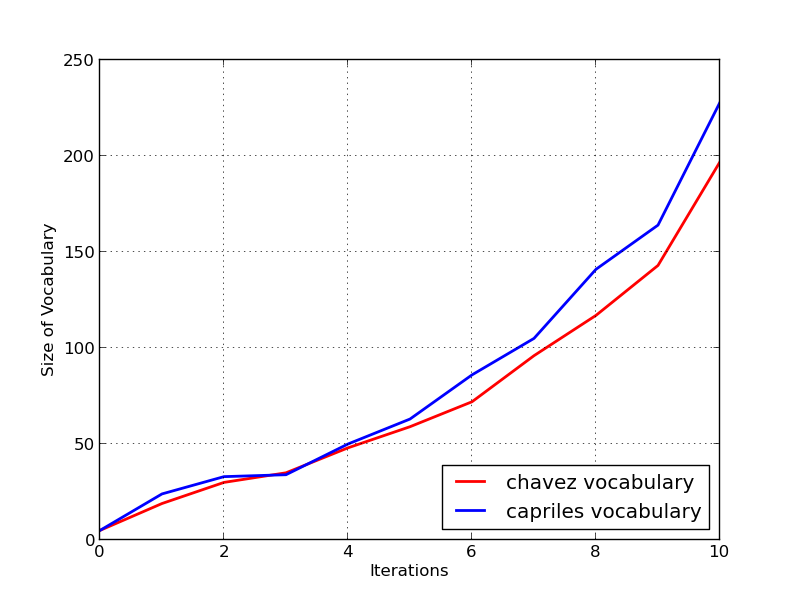
\includegraphics[scale=0.50]{support_files/WordGrowth.png}
	\caption{Vocabulary growth with each iteration.}
	\label{fig:wordgrowth}
\end{figure*}

The last two rules defined below encode the assumption that when two hashtags co-occur and one is a name of a candidate then the other hashtag is bound to be about the candidate too.
Since these two rules have two variables $\textsc{W1}$ and $\textsc{W2}$, the number for rules generated by substituting actual groundings (hashtags) increase rapidly with the number of tweets feeding into the inference process. 
This was a major contributing factor to the memory issues detailed in the optimal window size discussion.
\begin{align*}
\begin{split}
\textsc{Contains}(T,W1)
 \softand \textsc{Contains}(T,W2)
  \softand   \textsc{SeedWord}(W1,G)
  \softand \textsc{Positive}(T) \\
	\Rightarrow \textsc{Belongs}(W2,G)
\end{split}
\end{align*}
\begin{align*}
\begin{split}
\textsc{Contains}(T,W1) 
	\softand \textsc{Contains}(T,W2)
	\softand	 \textsc{SeedWord}(W1,G)
	\softand \textsc{Negative}(T)\\
	\Rightarrow \sim \textsc{Belongs}(W2,G)
\end{split}
\end{align*}
In addition to the rules, we also define constraints on the $\textsc{Belongs}$ and $\textsc{IsMember}$ predicates so that a particular hashtag or author can be associated to at most one candidate. 
Once all the tweets are loaded into the PSL program as predicates, we start the inference process by closing all the predicates except $\textsc{IsMember}$ and $\textsc{Belongs}$. 
This way, only the truth values of these two predicates are inferred and the other groundings of the closed predicates are regarded as facts.

\section{Results}
In this section we show how adept our PSL-based dynamic query expansion algorithm is at extracting relevant hashtags/keywords over the course of an election season.
Then in the fourth chapter we document how performance of forecasting algorithms improve using our expanded vocabularies.
\begin{figure*}
	\centering
	\subfloat[Day 0]
	{
		
\includegraphics[width=0.5\textwidth, height=0.35\textheight]{support_files/caprilesWordCloud1.png}
		\label{fig:wordCloud1}
	} 
	\subfloat[Day 6]
	{
		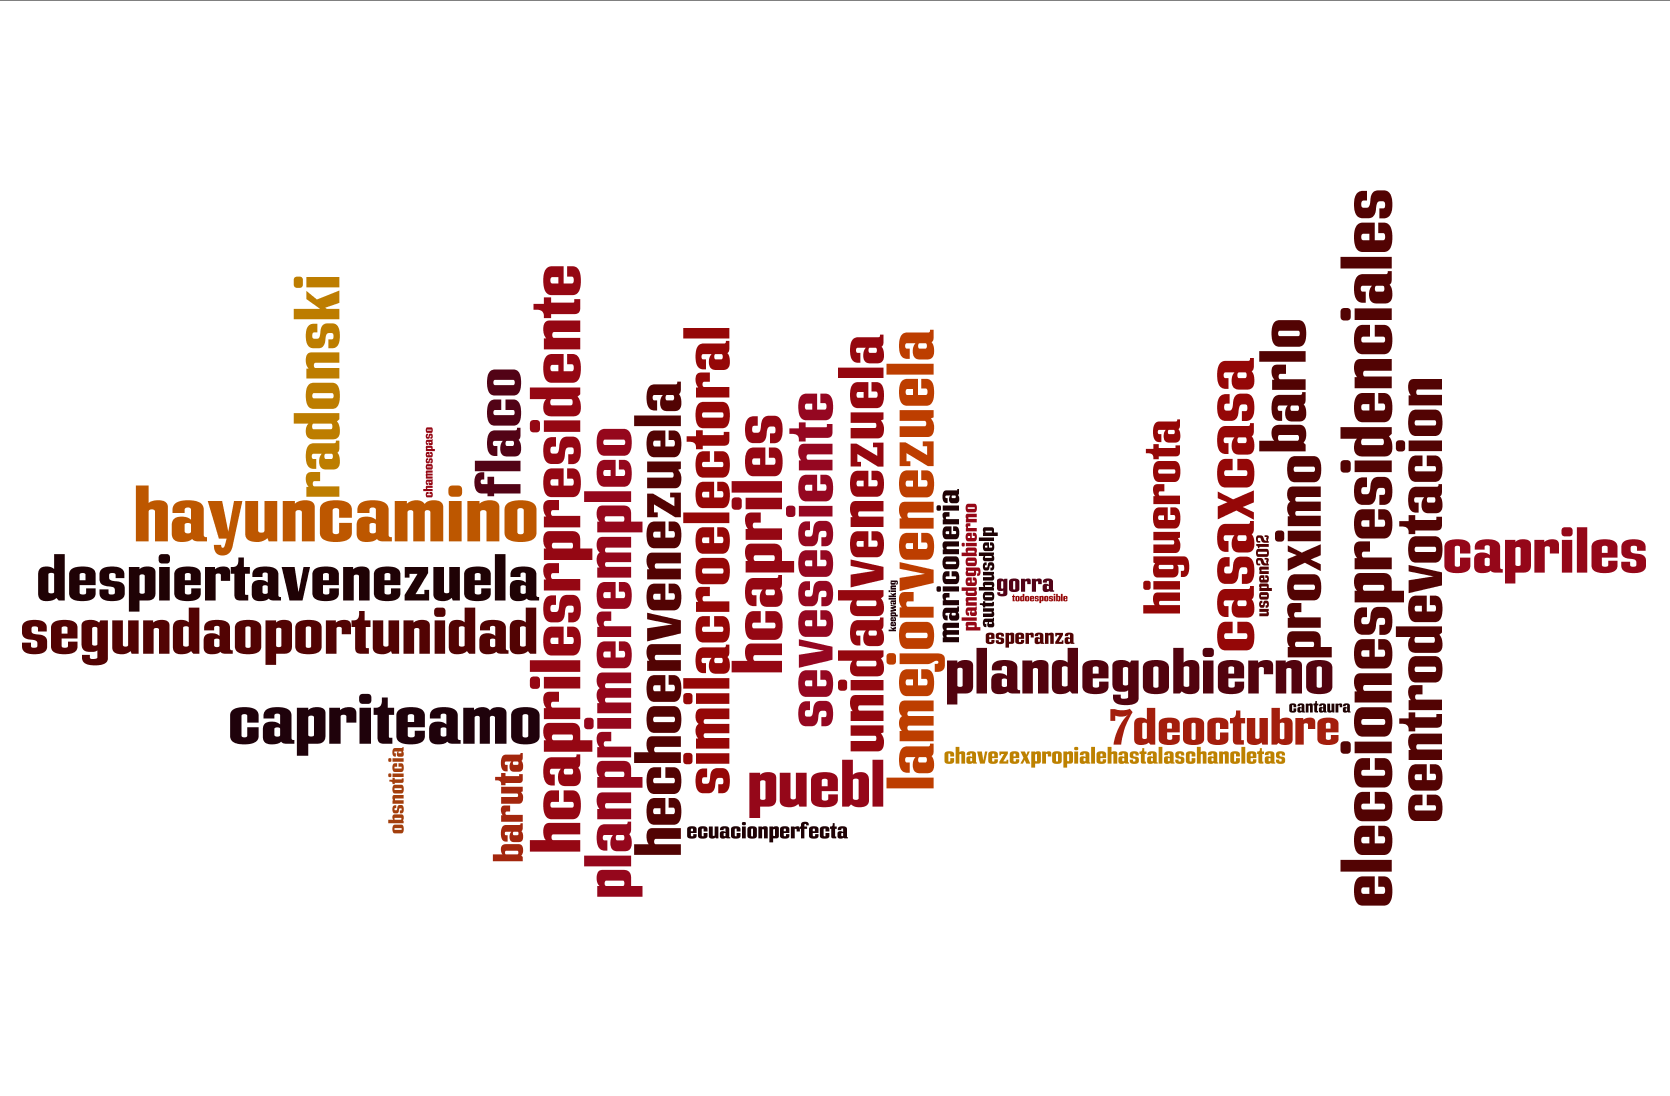
\includegraphics[width=0.5\textwidth, height=0.35\textheight]{support_files/caprilesWordCloud2.png}
		\label{fig:wordCloud2}
	} \\
	\noindent 
	\subfloat[Day 15]
	{
		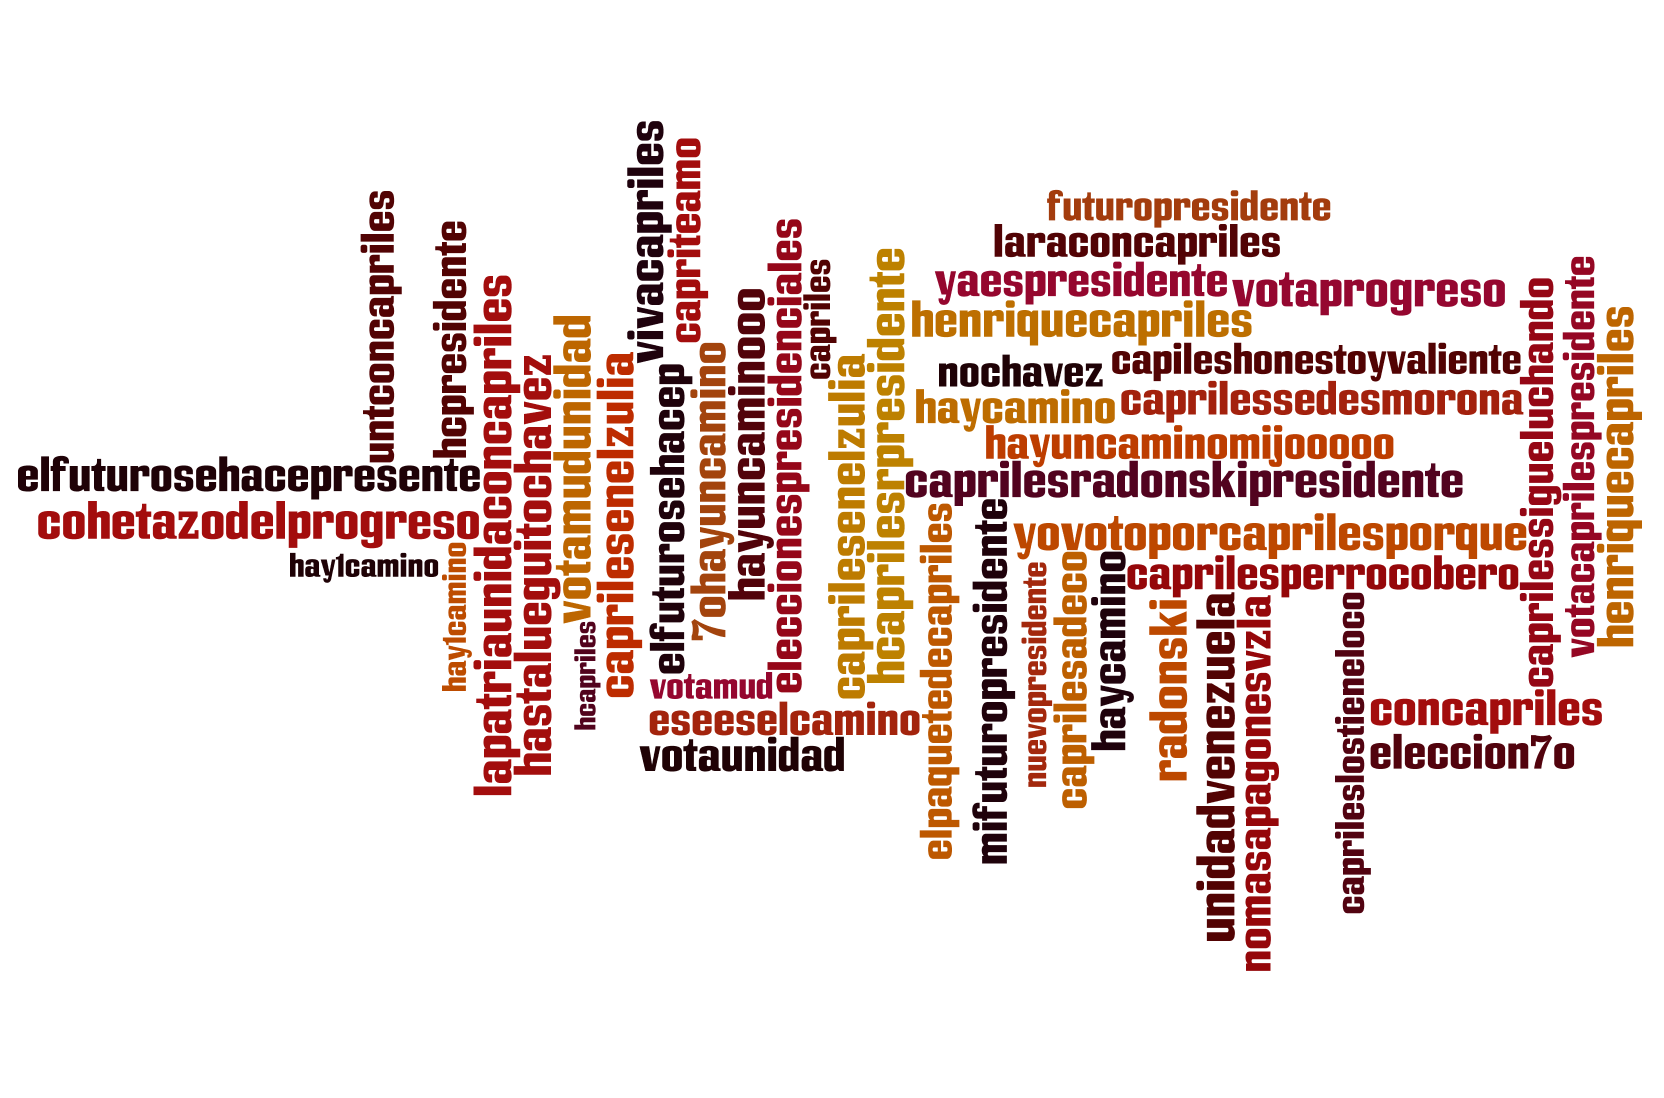
\includegraphics[width=0.5\textwidth, height=0.35\textheight]{support_files/caprilesWordCloud3.png}
		\label{fig:wordCloud3}
	}
	\subfloat[Day 30]
	{
		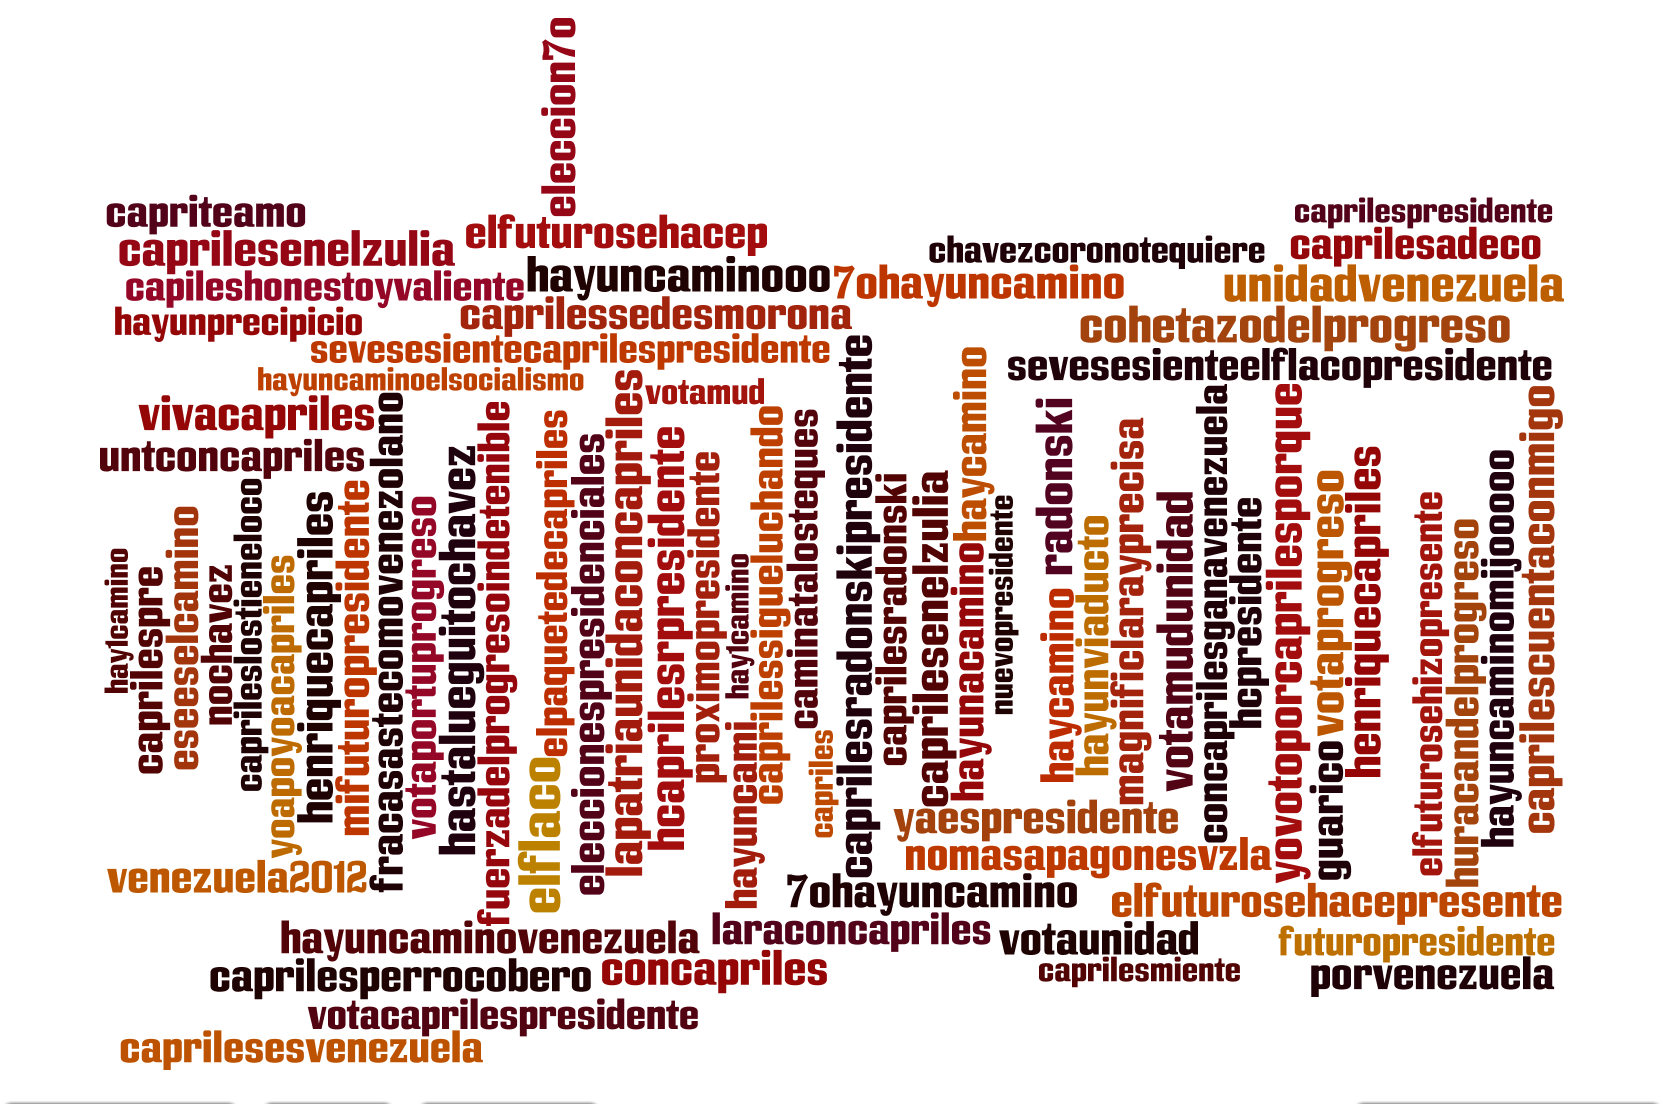
\includegraphics[width=0.5\textwidth, height=0.35\textheight]{support_files/caprilesWordCloud4.png}
		\label{fig:wordCloud4}
	}
	\caption{Evolution of hashtags for Henrique Capriles} 
	\label{fig:wordCloud}
\end{figure*}

\noindent
{\bf Venezuela:} \\
Figure~\ref{fig:wordgrowth} shows  how the vocabulary grows with each iteration for the two candidates who contested the Venezuelan presidential election on October 7th 2012.
Figure~\ref{fig:wordCloud} shows how the hashtags for Henrique Capriles evolved during the month leading up to the election.
Initially in Figure~\ref{fig:wordCloud1} the system begins with only a few hand picked hashtags that constitute the seed vocabulary. 
After a few iterations Figure~\ref{fig:wordCloud2} shows how the vocabulary has grown.
However, not all the words identified until now remain in the final vocabulary as the system drops certain words in successive iterations.
At the same time it is also noticed that hashtags like ``capriles" and ``hayuncamino" which are very strongly associated with Capriles consistently remain as the top ranked hashtags even after ten iterations (Figure~\ref{fig:wordCloud4}). 
It is also interesting to note that the algorithm identified hashtags like ``nochavez" (Figure\ref{fig:wordCloud3}) and attributed it rightly to Hugo Ch\'{a}vez's primary contender, i.e., Capriles. \\
\begin{figure*}[Ht]
	\centering
	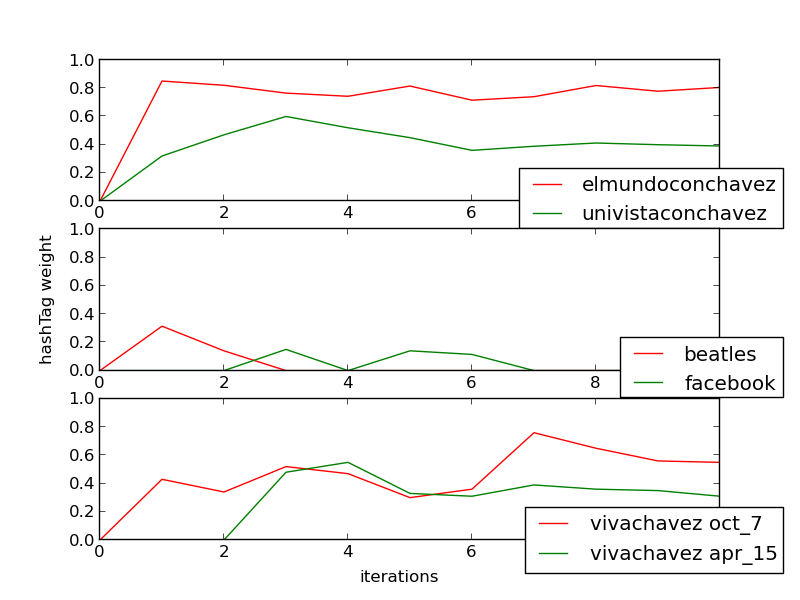
\includegraphics[scale=0.65]{support_files/hashTagTimeSeries.png}
	\caption{Time series comparison for different hashtags identified for Hugo Cha\'{a}vez.}
	%The first plot shows "univistaconchavez" and "elmundocochavez". The second plot shows "Beatles" and "Facebook". The third plot shows "vivachavez" from two different elections conducted on 15th April 2013 and 7th October 2012.
	\label{fig:timeSeries}
\end{figure*}
In Figure~\ref{fig:timeSeries}, the first plot elucidates how hashtags like \emph{``elmnduconchavez"} and 
\emph{``univistaconchavez"} remain highly associated with Hugo Ch\'{a}vez for the October 7th Presidential election. 
These hashtags remain indicative of a user's affiliation throughout the month leading up to the election.
Meanwhile hashtags such as \emph{"beatles"} and \emph{"facebook"} (in second plot) show spikes in their time series primarily because users affiliated with Ch\'{a}vez used them during that time window. 
But as the iterative process continues, the system drops these non-informative words.
The third plot presents another interesting observation.
Hugo Ch\'{a}vez who had won the election on October 7, 2012 was diagnosed with cancer and passed away
before being sworn in as the President.
This triggered a re-election on April 15, 2013 where Nicolas Maduro, who had assumed the role of acting president then, competed 
against Henrique Capriles in the Presidential race.
The hashtag \emph{``vivachavez"} is part of both the elections, despite the 
fact that Hugo Ch\'{a}vez did not compete in the second election.
It is picked up as a phrase commonly used by supporters of Nicholas Maduro whose election campaign was strategized around the death of Hugo Ch\'{a}vez to garner sympathy and mobilize support.
Similarly variations of the hashtags \emph{``hayuncamino"} and \emph{``unidadvenuzela"} were returned 
for Henrique Capriles for both these elections.
The tag MUD is for ``Mesa de la Unidad Democratica” (Democratic Unity Roundtable) that was the organization created for the opposition to Ch\'{a}vez. 
The vocabulary grows to include other terms associated to the campaign, as the official slogan for the opposition ``hayuncamino” (there is a road). 
Others relate to programs that Capriles wanted to implement, such as ``planprimerempleo” (First Job Program). 

\begin{figure*}
	\centering
	\subfloat[Nov 24]
	{
		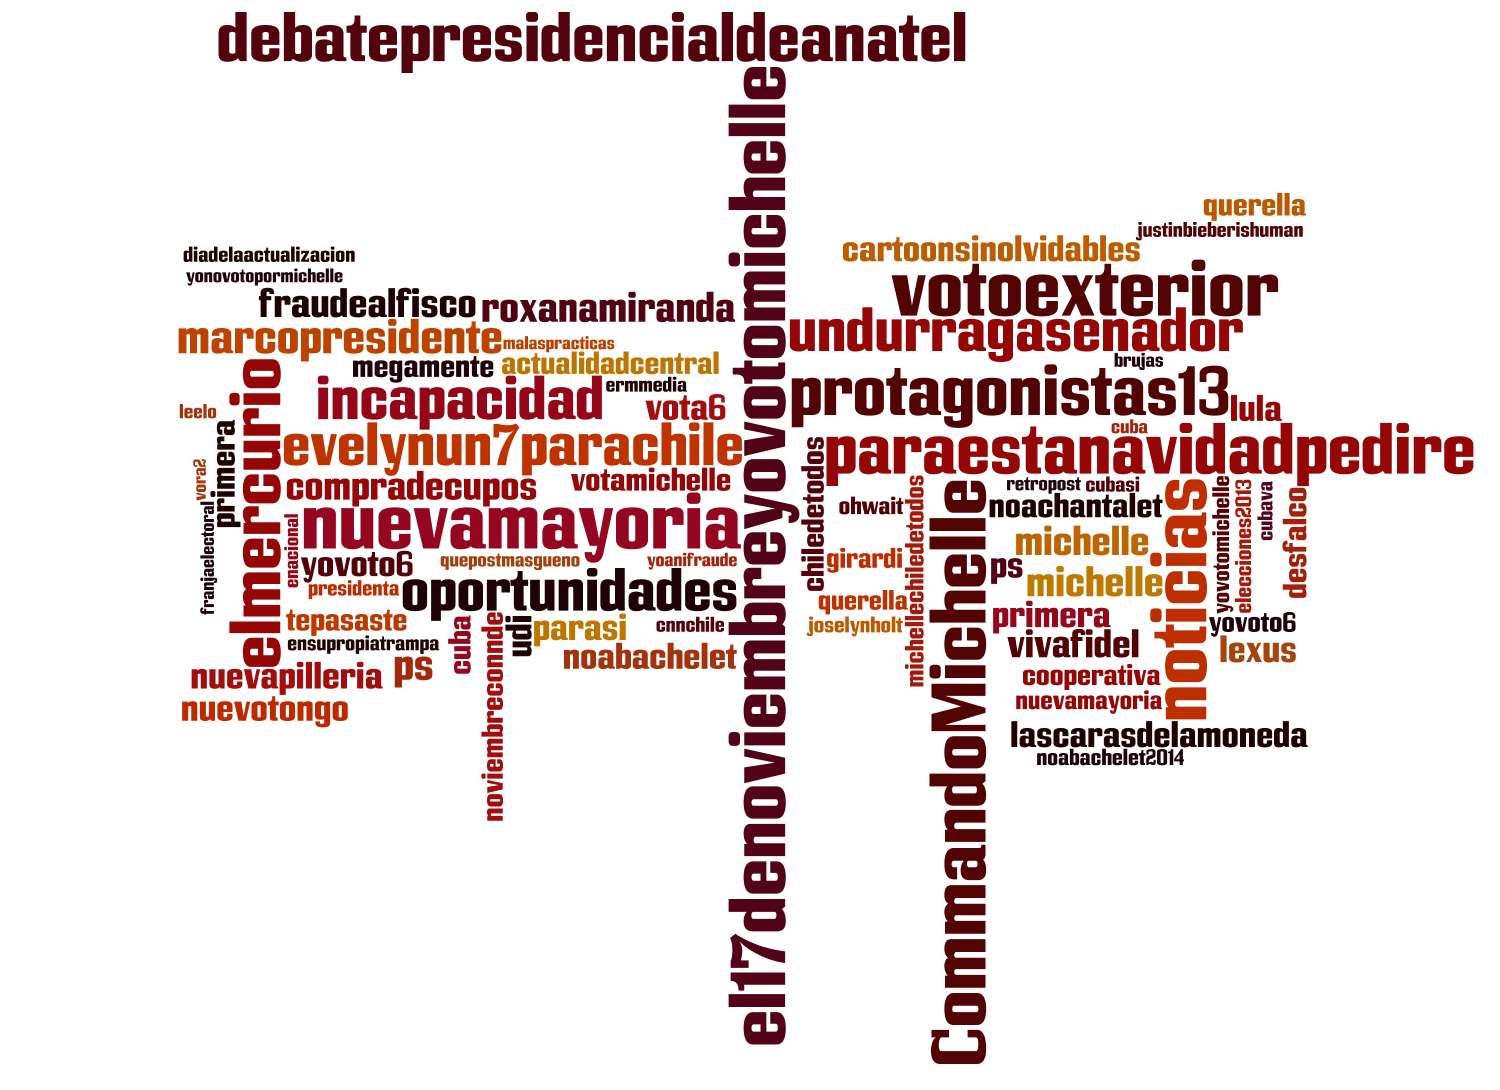
\includegraphics[width=0.5\textwidth, height=0.35\textheight]{support_files/bacheletWordCloud1.png}
		\label{fig:bacheletwordCloud1}
	} 
	\subfloat[Dec 15]
	{
		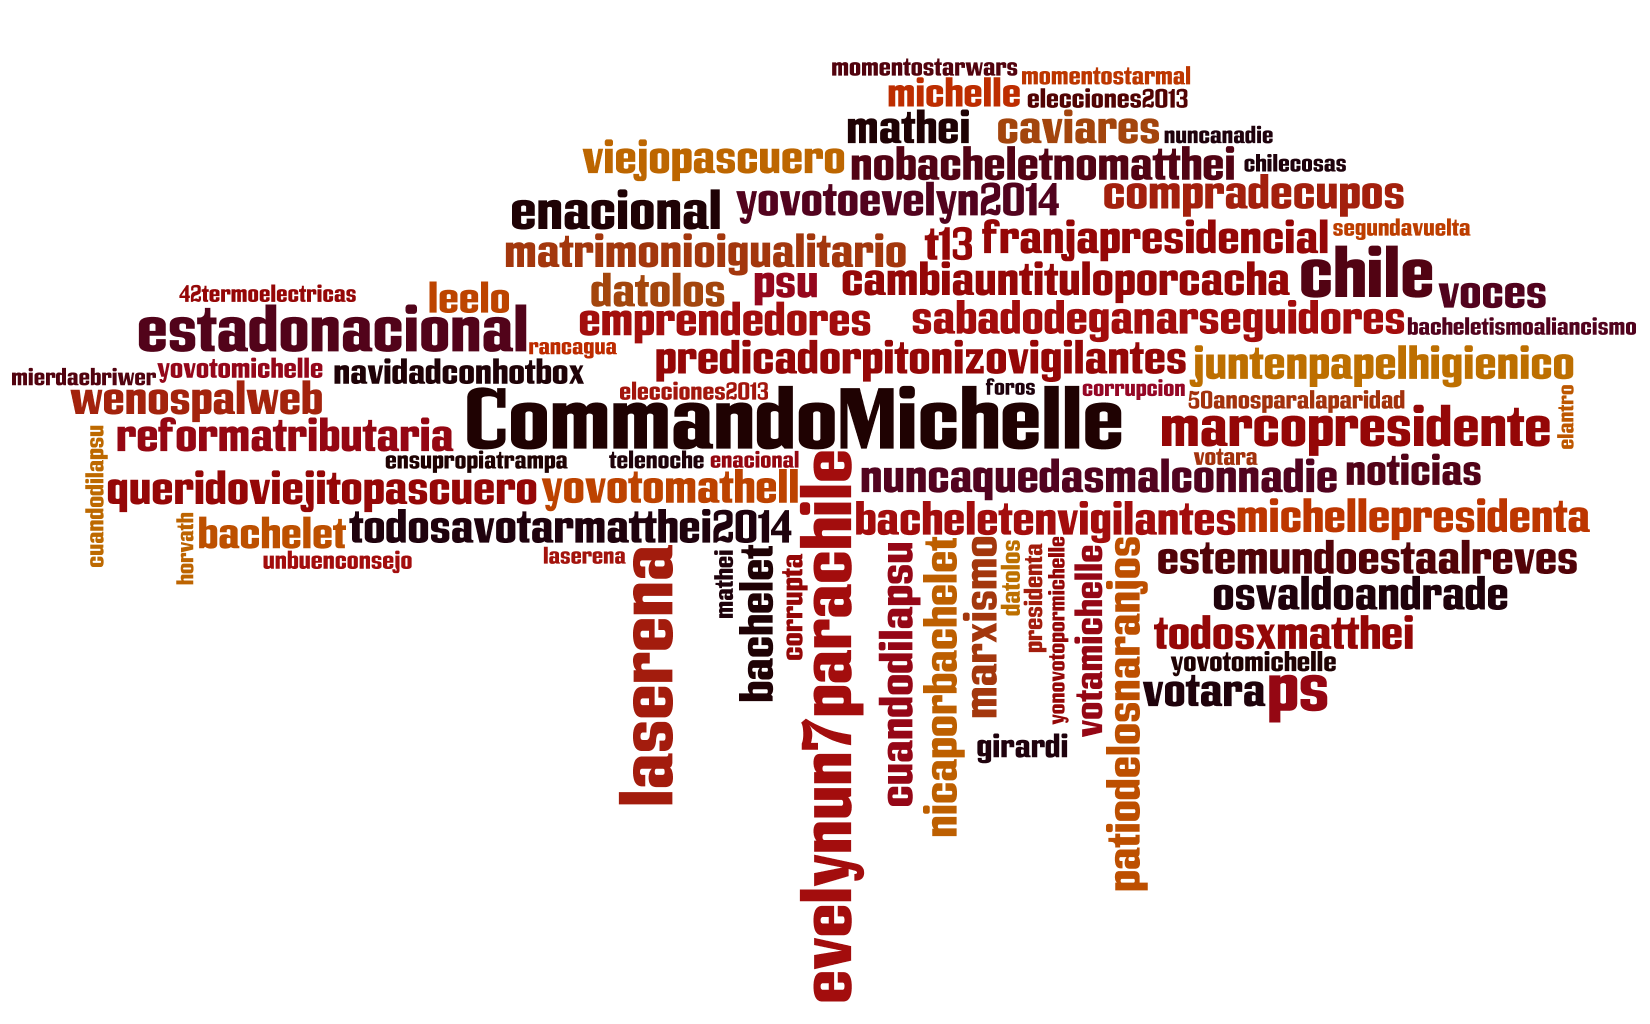
\includegraphics[width=0.5\textwidth, height=0.35\textheight]{support_files/bacheletWordCloud2.png}
		\label{fig:bacheletwordCloud2}
	}
	\caption{Hashtags identified for Michelle Bachelet} 
	\label{fig:bacheletwordCloud}
\end{figure*}

\noindent
{\bf Chile:}
Figure~\ref{fig:bacheletwordCloud} shows the hashtags identified for Michelle Bachelet who won the Chilean Presidential elections that was decided over two rounds.
The first round was conducted on the 24th of November, 2013 and the 2nd round was conducted on December 15, 2013. 
The query expansion pipeline for Bachelet's group in both these elections were initialized only with three seed words: {\it Bachelet, CommandoMichelle} and {\it PS}. 
The first name of the candidate was not used as it introduced a lot of noise because ``Michelle" is a very common name.
The first figure shows the hashtags identified for Bachelet during the first round and the second figure for the second round. 
It can be seen that there is a lot of overlap in the vocabulary which is the expected outcome. 
Similarly there were a lot of common hashtags between the two rounds of election for the other candidate, Evelyn Matthei, too.
\begin{figure*}[scale=0.75]
	\centering
	\subfloat[Mexico]
	{
		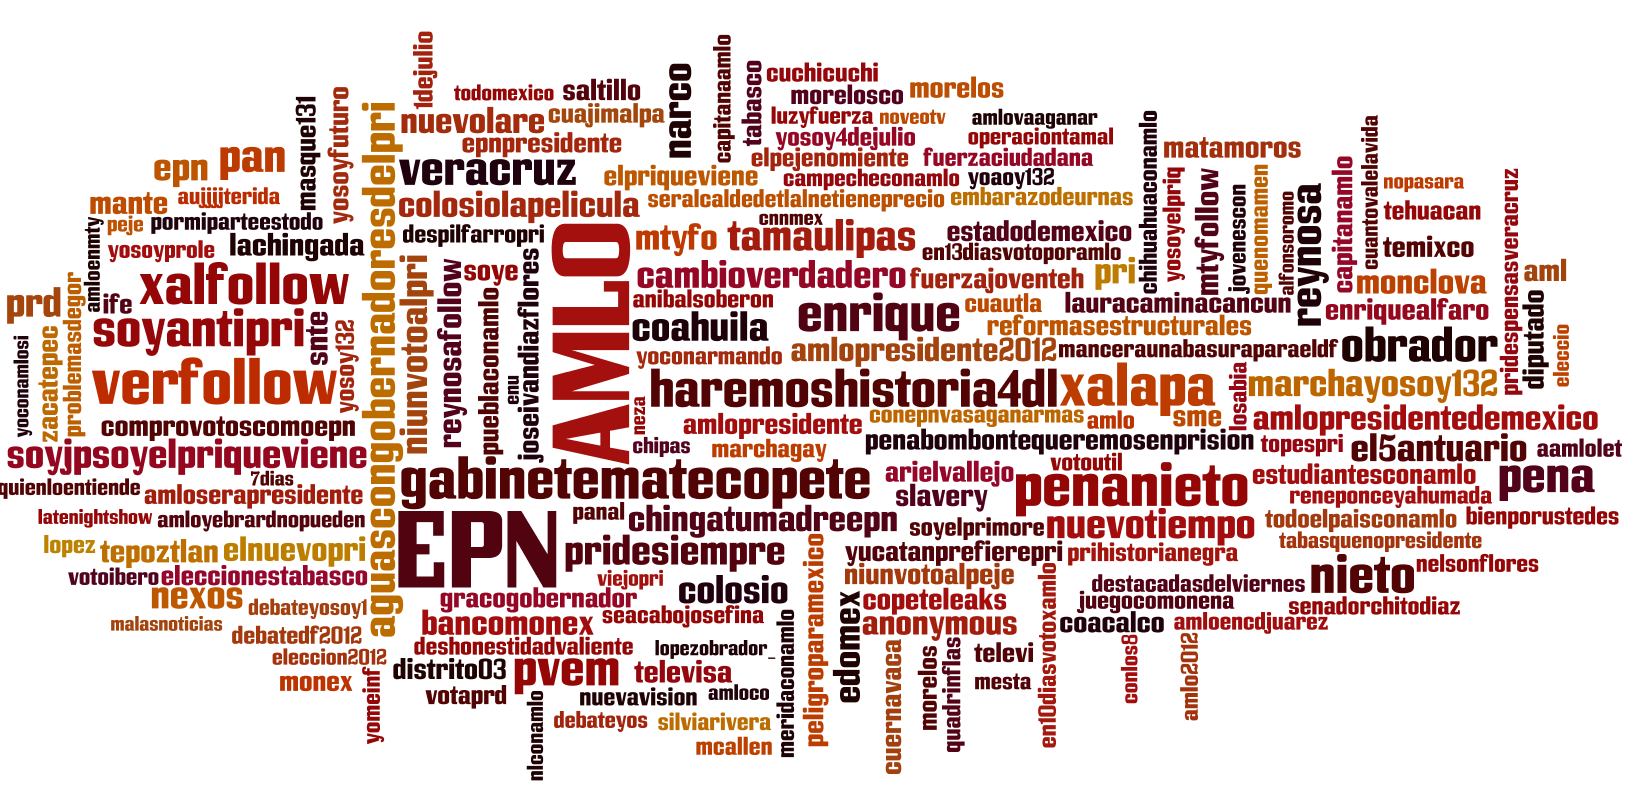
\includegraphics[width=0.5\textwidth, height=0.40\textheight]{support_files/mexicoWordCloud.png}
		\label{fig:mexicowordCloud}
	} 
	\subfloat[Paraguay]
	{
		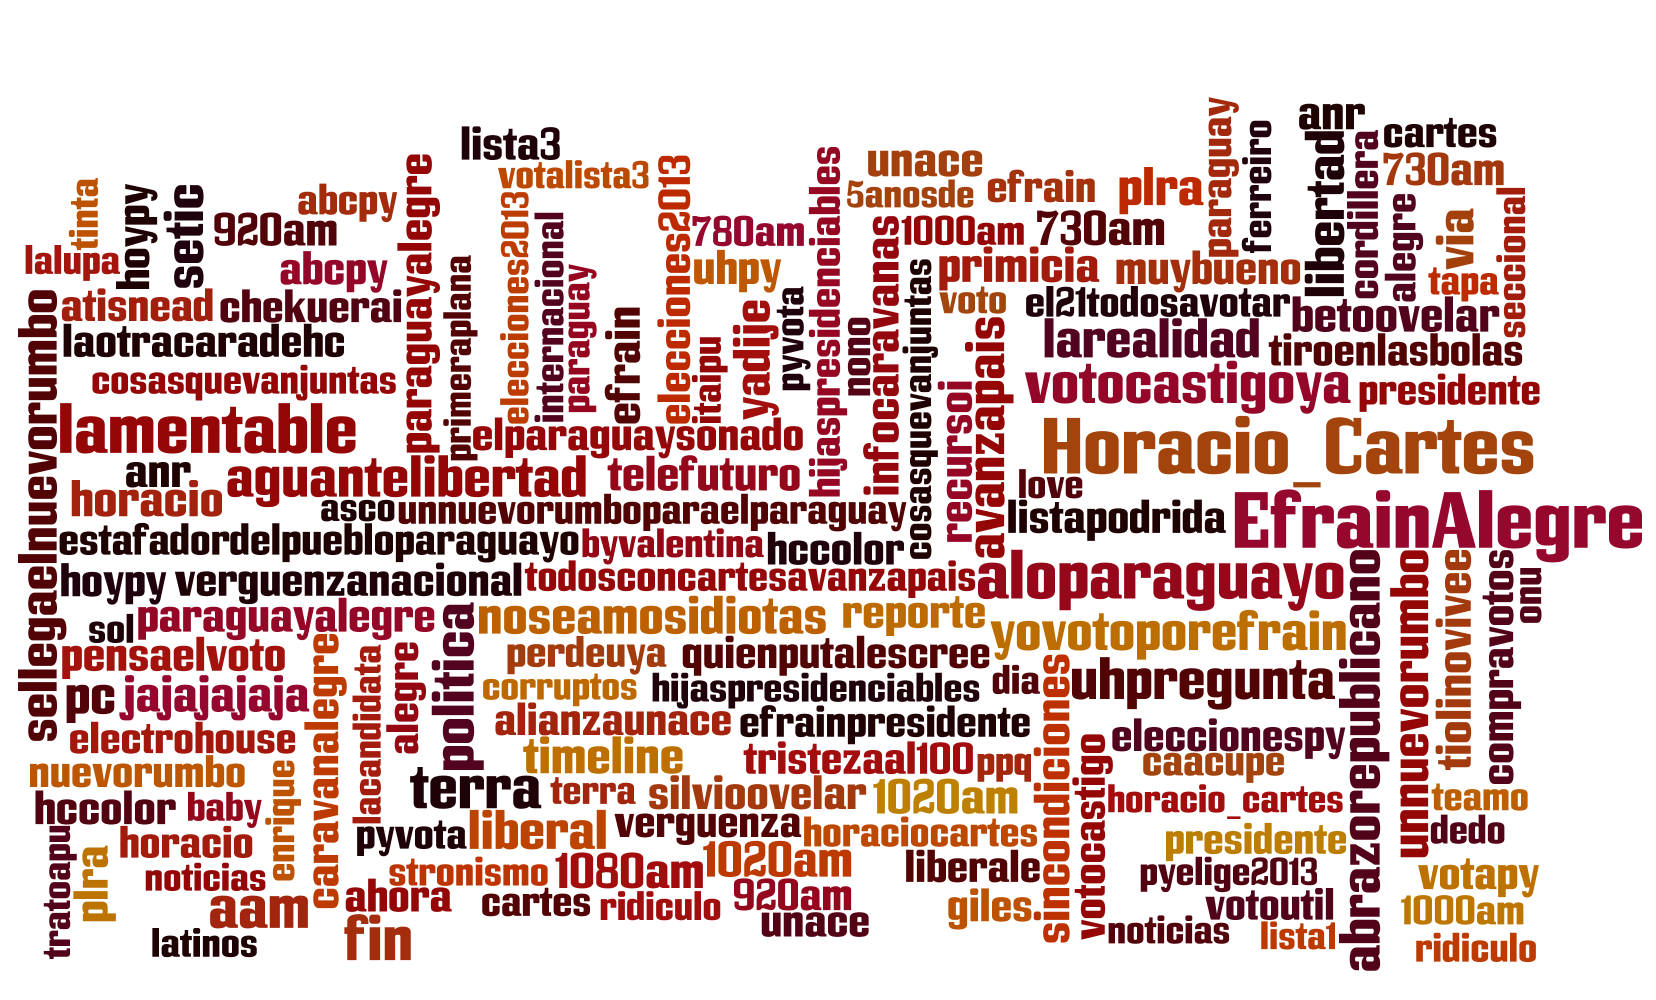
\includegraphics[width=0.5\textwidth, height=0.40\textheight]{support_files/paraguayWordCloud.png}
		\label{fig:paraguaywordCloud}
	} \\
	\noindent 
	\subfloat[Honduras]
	{
		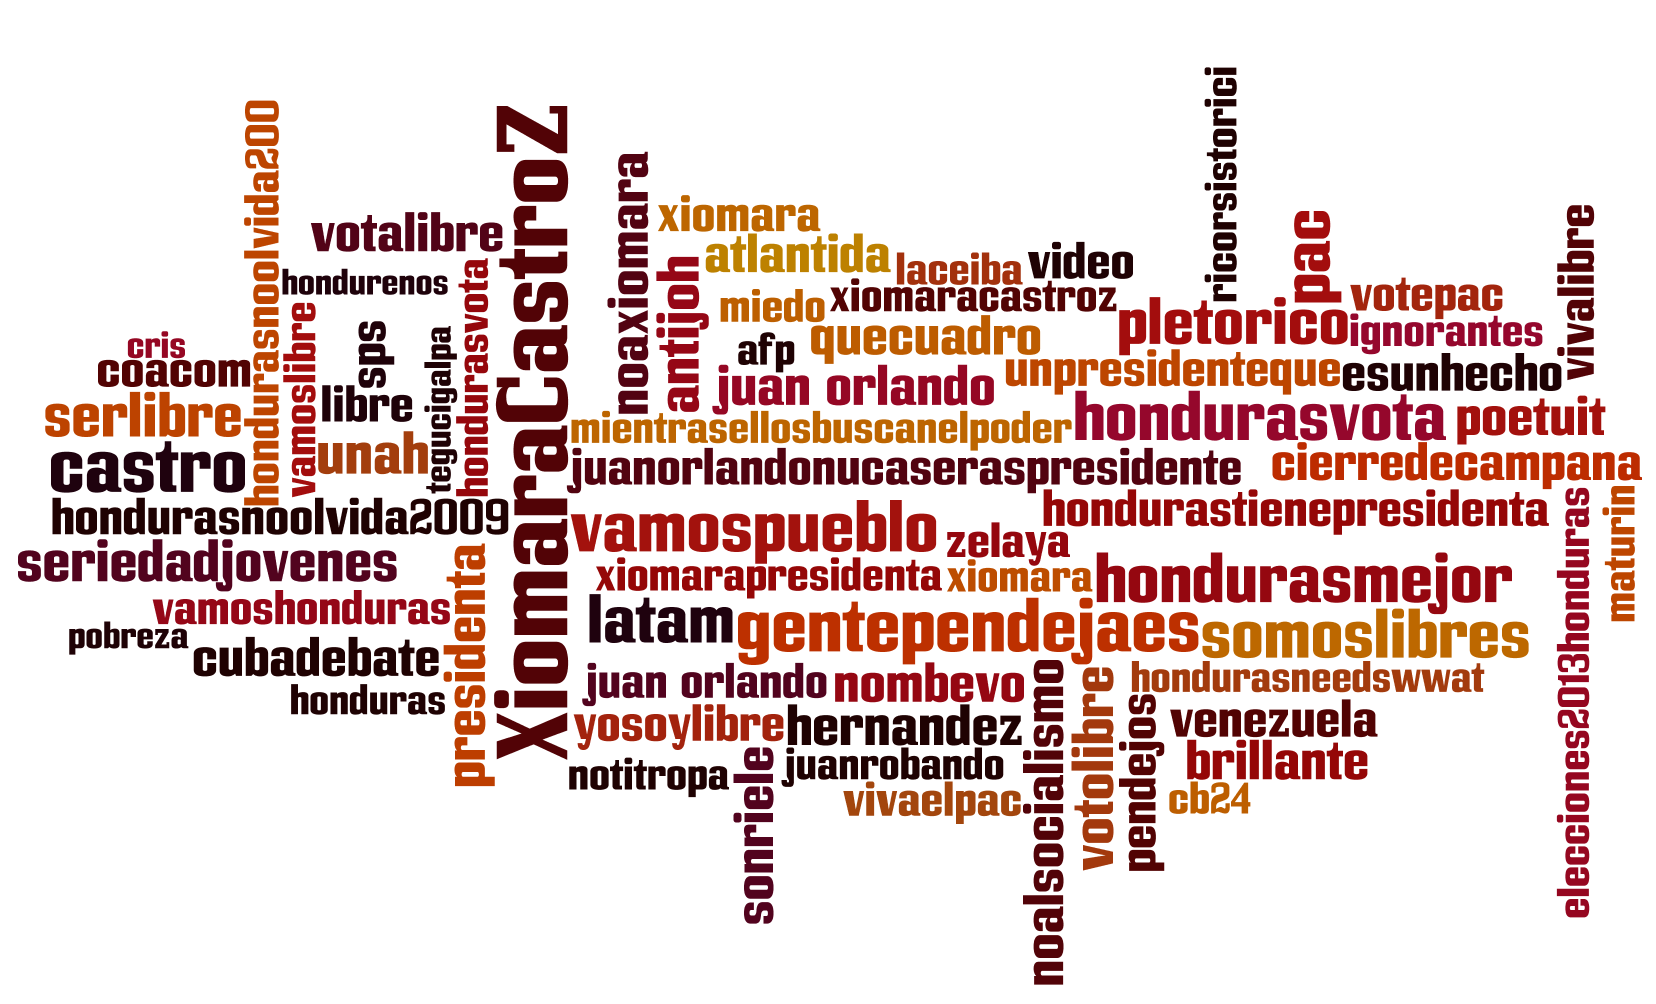
\includegraphics[width=0.5\textwidth, height=0.40\textheight]{support_files/hondurasWordCloud.png}
		\label{fig:honduraswordCloud}
	}
	\subfloat[Ecuador]
	{
		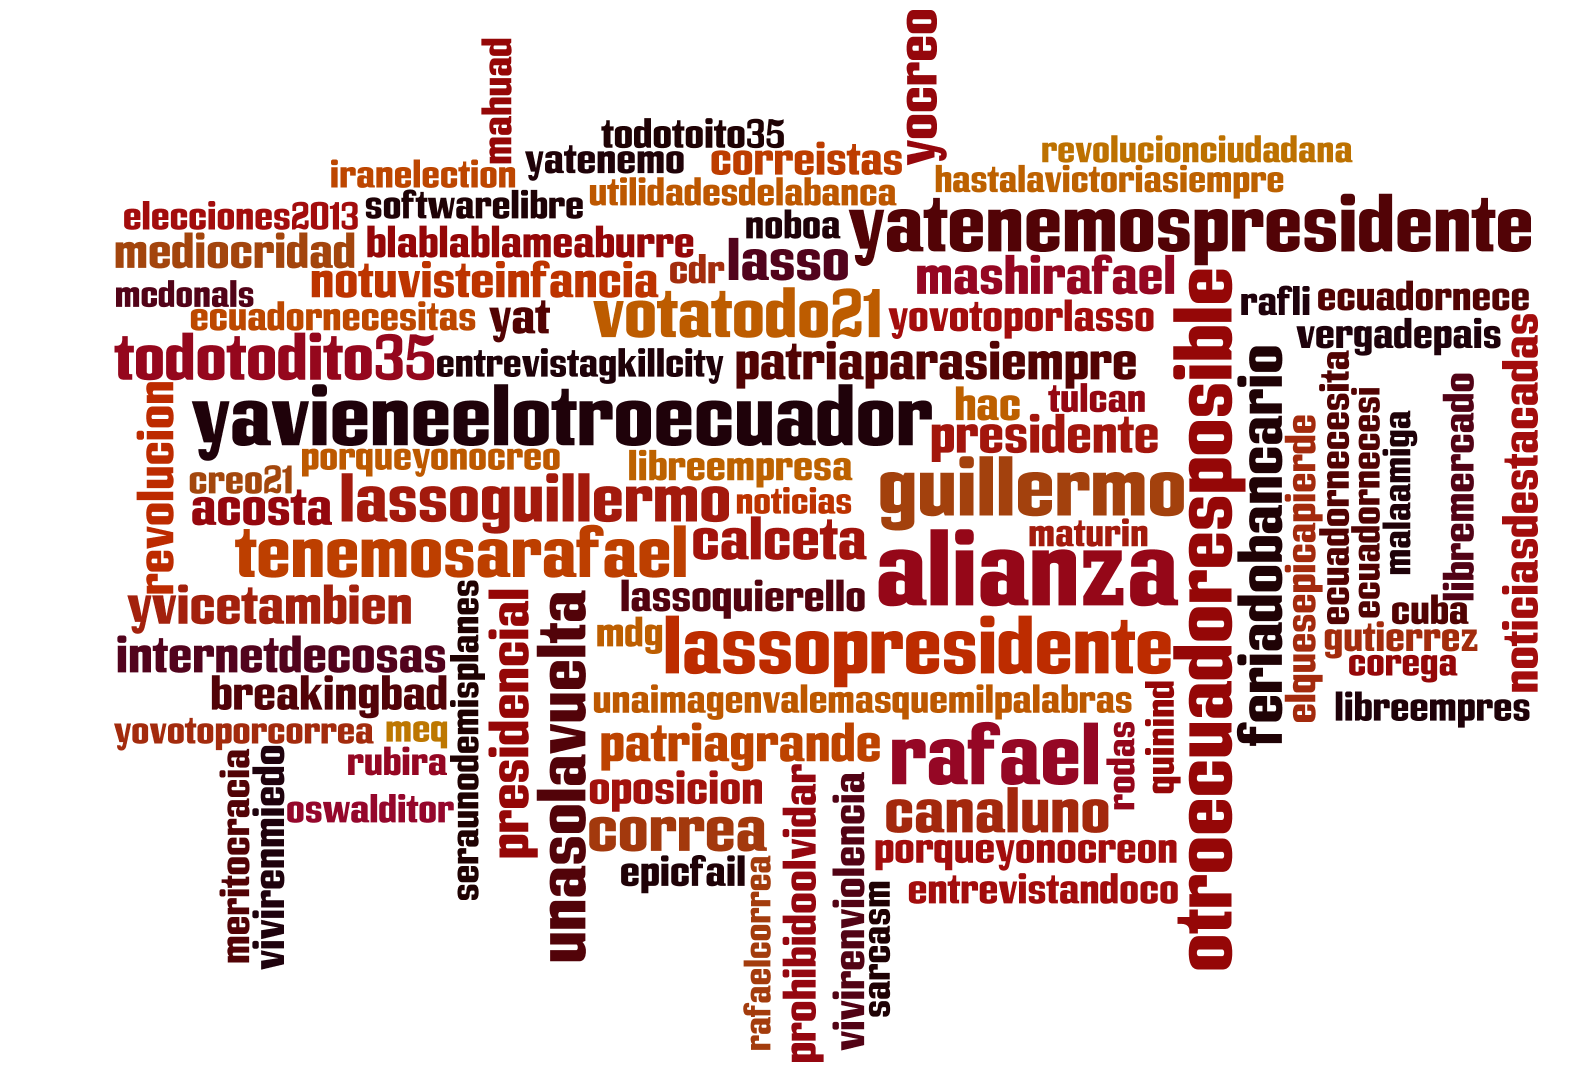
\includegraphics[width=0.5\textwidth, height=0.40\textheight]{support_files/ecuadorWordCloud.png}
		\label{fig:ecuadorwordCloud}
	}
	\caption{Vocabulary of hashtags identified for different elections} 
	\label{fig:countrywordCloud}
\end{figure*}

Figure~\ref{fig:countrywordCloud} shows the hashtags identified for the elections from Mexico, Paraguay, Honduras and Ecuador.\\
\noindent	
{\bf Mexico:} A general election in Mexico took place on July 1st, 2012.
The two front runners where Enrique Pe\'{n}a Nieto (EPN) and Andres Manuel L\'{o}pez Obrador (AMLO).
The tags (Figure~\ref{fig:mexicowordCloud}) show the contest between these two candidates, the first belonging to the “Partido Institucional Revolucionario” (PRI). 
Among the tags we can also find reference to the “yosoy132” student movement that became a key player during the election. 
%We have against AMLO some as “niunvotoalpeje” (no one vote for AMLO) or against EPN “soyantipri” (I am against PRI).
We also see “niunvotoalpeje” (no one vote for AMLO) and “soyantipri” (I am against PRI) which are attributed against AMLO and EPN respectively.

\noindent
{\bf Paraguay:}
Figure~\ref{fig:paraguaywordCloud} details the election between Horacio Cartes from the Partido Colorado and Efrain Alegre from Alianza Paraguay. 
The incumbent president belonged to Partido Colorado and we can see some tags talking about a protest vote: “votocastigoya” (protest vote now). 
Also references from their campaign to each candidate as “yovotoporefrain” (I vote for efrain) or “todosconcartesavanzapais” (everyone with cartes, the country goes forward) are seen.

\noindent
{\bf Honduras:}
In November 2013 Honduras had a general election to choose President, Congress and local officials. 
The wife of former President Zelaya, Xiomara Castro, contended against Juan Orlando Hernandez from the incumbent Partido Nacional. 
Both candidates showed similar numbers in the polls before the election. 
We can find tags that either support Xiomara, like “xiomarapresidenta” (Xiomara President), “hondurastienepresidenta” (Honduras has a female president) or against her, “noaxiomara” (no to Xiomara) in Figure~\ref{fig:honduraswordCloud}.

\noindent
{\bf Ecuador:}
Ecuador had a first round for the presidential election on February 17th, 2013 where Rafael Correa obtained more than 50\% of the votes needed to avoid a second round. 
From the tags(Figure~\ref{fig:ecuadorwordCloud}) we can read support in phrases such as “yatenemospresidente” (we have elected president) or “tenemosarafael” (we have Rafael). 
There are some references to other candidates such as “lassopresidente” (candidate Lasso president).

It can be noticed that the vocabulary for the Honduran and Ecuadorean  elections are quite noisy. 
This is primary because Twitter is not as popular in these two countries as in Venezuela or Chile and therefore the number of tweets
used for the inference was significantly lesser.
This in turn affected the PSL inference mechanism as the lack of evidence pushed the weights for the hashtags down.
Therefore, the threshold value in the post processing step was set lower than normal to avoid losing the informative words.
But this in turn also introduced a bit of noise to the vocabulary.